\documentclass[reqno,12pt,notitlepage]{article}
\usepackage{amsmath}
\usepackage{amsthm}
\usepackage{amssymb}
\usepackage{setspace}
\usepackage{graphicx}
\usepackage{booktabs}
\usepackage{pdflscape}
\usepackage{url}
\usepackage{caption}
\usepackage{multirow,rotating,multicol}
\usepackage{listings}
\usepackage[bookmarks,hidelinks]{hyperref}
\usepackage{longtable}
\usepackage{threeparttable}
%\usepackage[position=top, font=normalsize]{subfig}
\usepackage{subcaption}
\usepackage{caption}
\usepackage{float}
\usepackage{pgfpages,tikz}
\usepackage{adjustbox}


% modifications
\newtheorem{proposition}{Proposition}
\DeclareMathOperator*{\plim}{plim}

\newcommand{\question}[1]{ \begin{center} \noindent\colorbox{gray!8}{
\parbox{0.8\textwidth}{\vspace{0.125in} #1 \vspace{0.125in} } } \end{center} }

\newcommand{\EE}{\mathbb{E}}
\newcommand{\PP}{\mathbb{P}}

\newcommand{\var}[1]{\operatorname{Var}\left( #1 \right)}
\newcommand{\cov}[1]{\operatorname{Cov}\left( #1 \right)}


% hyperref settings
\hypersetup{%
   colorlinks=false
}

% geometry
\usepackage[left=1in, right=1in, top=1in, bottom=1in]{geometry}

% bib
\usepackage[round]{natbib}


% paragraphs
\setlength{\parindent}{0pt}
\setlength{\parskip}{12pt}

\usepackage{color}
\usepackage{hyperref}
\hypersetup{
    colorlinks=true, % make the links colored
    linkcolor=blue, % color TOC links in blue
    citecolor=blue, %citation colors blue
    urlcolor=red, % color URLs in red
    linktoc=all % 'all' will create links for everything in the TOC
}


\title{Topics in Econometrics - Assignment 1}
\author{Yixin Sun}
\date{\today}

\begin{document}

\maketitle

\section*{Question 1b and 1c}
We see here that the average $\hat{\beta}_{1}$ is about the same as the true $\beta_1$. The variance of the estimate decreases from $p =1$ to $p = 5$, and then increases after that. This makes sense as the $p=1$ regression suffers from omitted variable bias, whereas $p >5$ is overfitting with variables that are not actually related to the outcome variable or explanatory variable of interest. Even if you included the regressors that are independent of the one you care about, these independent regressors interfere. 

\begin{table}[H]
    \centering
    \caption{Average and Variance of $\hat{\beta}_1$}
    
\begin{tabular}{rrr}
\toprule
p & mean & variance\\
\midrule
1 & 1.003 & 0.020\\
5 & 1.000 & 0.009\\
10 & 1.000 & 0.010\\
50 & 1.000 & 0.018\\
85 & 1.011 & 0.065\\
\addlinespace
90 & 1.010 & 0.102\\
\bottomrule
\end{tabular}

\end{table}


\section*{Question 1d}
\begin{table}[H]
    \centering
    \caption{Frisch-Waugh-Lovell Results}
    
\begin{tabular}{rrr}
\toprule
p & x1\_2 & x\_eigen\\
\midrule
5 & 0.041 & 74.175\\
10 & 0.091 & 55.700\\
50 & 0.491 & 10.487\\
85 & 0.840 & 0.965\\
90 & 0.892 & 0.495\\
\bottomrule
\end{tabular}

\end{table}
This table shows that the value of the lowest eigenvalue decreases as the number of regressor increase, while $1 / N \sum_{i} \hat{X}_{i 1}(\tilde{p})^{2}$ increases as we add more regressors. $1 / N \sum_{i} \hat{X}_{i 1}(\tilde{p})^{2}$ here is the variance of $\hat{X}_{i 1}$. 


We're thinking about what this $\tilde{p-1}$ unrelated regressors are doing to the estimation of $\beta_1$, the fitted value of th first regressor we care about. In the DGP, they are all independent regressors, so $\hat{X}_{1}$ should be zero. But as you add more independent regressors, the estimate gets worse, and hence the variance increases. The lowest eigenvalue addresses the invertibility of the regressors - the lowest eigenvealue is closer to the zero and there is more noise in the inverse. This is the same thing as variance of $\hat{X}_{i 1}$ getting bigger, which we see in the second column of table 2. 


\section*{Question 1e}
This is even worse than b, c, d. As $\rho$ and $N$ increase, the variance of $\hat{\beta}_1$ increases. The issue here is that the extra covariates are not actually correlated to $Y_1$. However, the correlation between the extra covariates and $X_1$ is causing the extra covariates to essentially steal variation that should be attributed to $X_1$, leading to more noise on the parameter of interest, $\hat{\beta}_1$.
\begin{table}[H]
    \centering
    \caption{Dependence Structure Between Covariates}
    
\begin{tabular}{rrrrr}
\toprule
mean $\beta_1$ & var $\beta_1$ & eig & N & $\rho$\\
\midrule
1.010 & 0.115 & 0.421 & 100 & 0.0\\
0.986 & 0.227 & 0.207 & 100 & 0.5\\
1.032 & 1.097 & 0.043 & 100 & 0.9\\
1.002 & 0.010 & 23.627 & 200 & 0.0\\
0.999 & 0.017 & 11.887 & 200 & 0.5\\
\addlinespace
0.991 & 0.088 & 2.386 & 200 & 0.9\\
1.001 & 0.002 & 172.734 & 500 & 0.0\\
1.000 & 0.005 & 86.569 & 500 & 0.5\\
1.007 & 0.025 & 17.328 & 500 & 0.9\\
1.001 & 0.001 & 502.059 & 1000 & 0.0\\
\addlinespace
1.001 & 0.002 & 252.314 & 1000 & 0.5\\
1.009 & 0.011 & 50.382 & 1000 & 0.9\\
\bottomrule
\end{tabular}

\end{table}

\section*{Question 1f}
When $\rho = 0$, there is no relationship between the covariates, and the eigenvalues decrease smoothly, since each additional coviariate adds unexplained variation to the set. However, when we do have correlation between covariates, we see that the eigenvalue starts off very high, and then immediately drops off. This shows the problem of collinearity: even if we have all these extra covariates, the strong correlation between them means that many do not hold any additional information.

\begin{figure}[H]
    \centering
    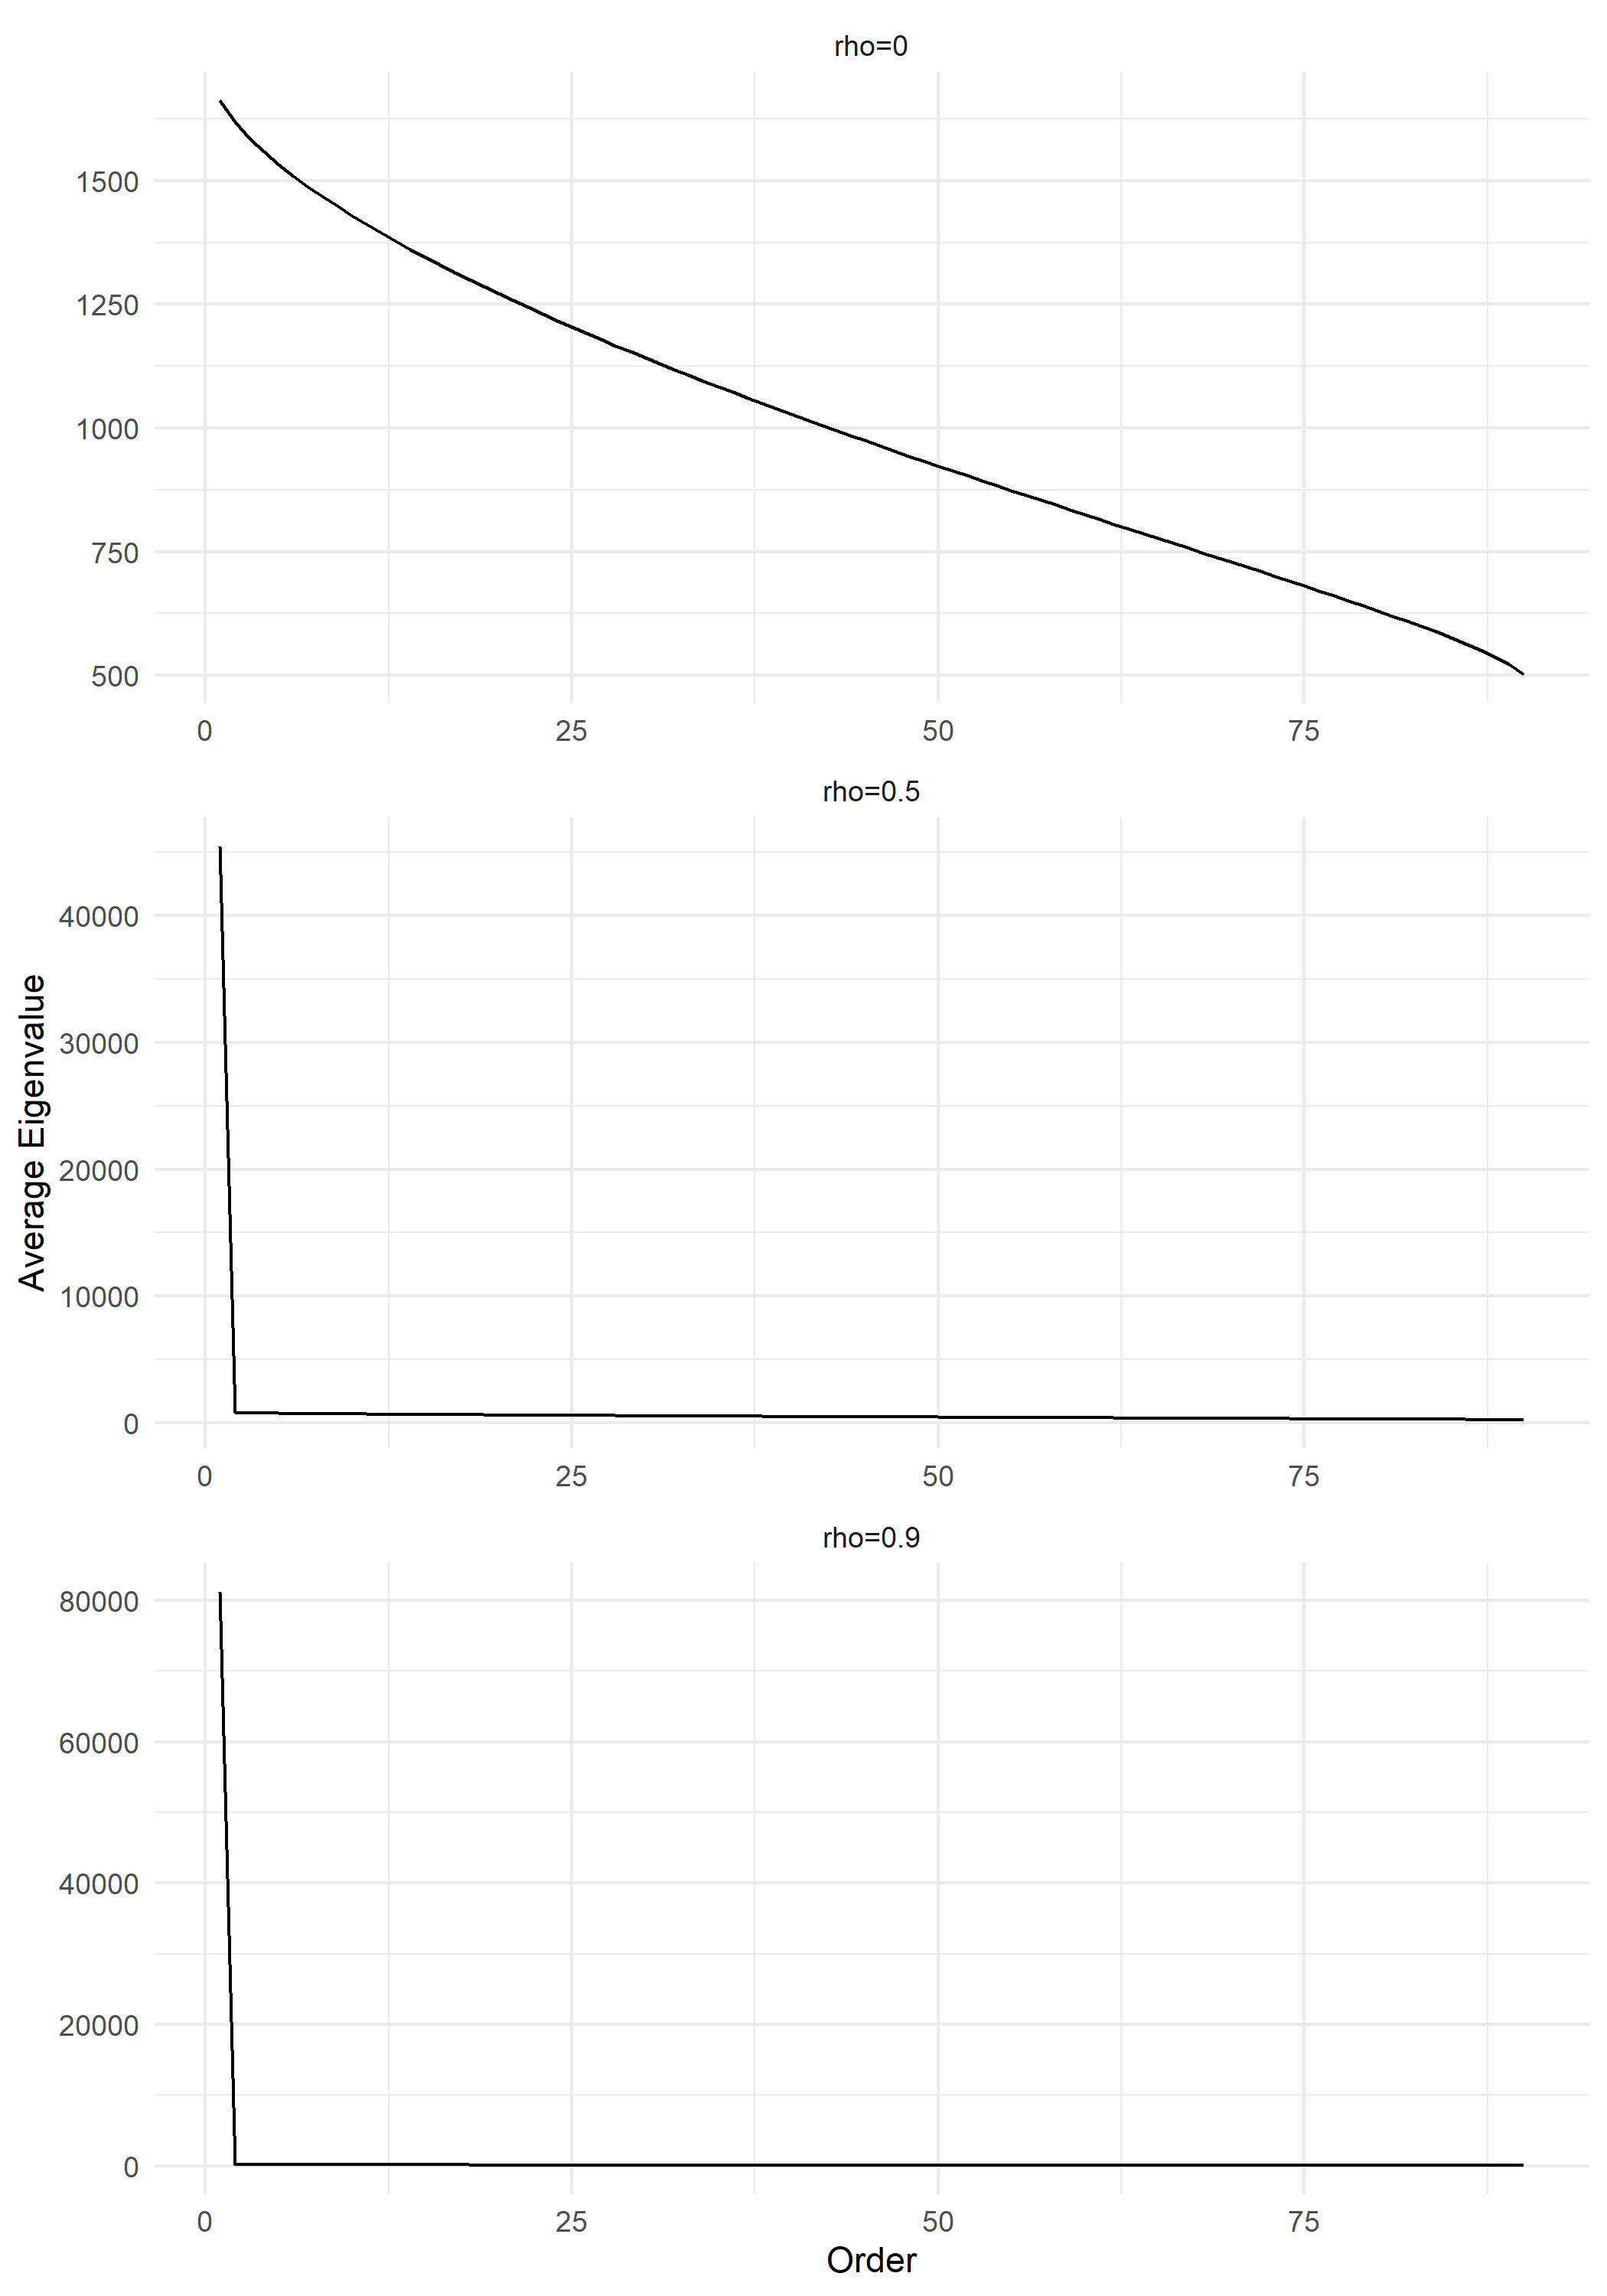
\includegraphics[width=.6\textwidth]{part_f.png}
\end{figure}

\newpage
\section*{Question 1g}

We see a similar relationship between $\rho$, $N$ and the variance of $\hat{\beta}_1$, but we see what happens with two different rates of convergence of $\frac{p}{N}$. When $p=0.9N$, $\lim_{N\rightarrow \infty} \frac{p}{N} = 0.9$. Thus we see in Table 4 that when $N$ increases, we do not see a huge impact on the lowest eigenvalue. When $p=20\times log(N)$, $\lim_{N\rightarrow \infty} \frac{p}{N} = 0$. We see that in Table 5, the eigenvalues increase dramatically as $N$ increases, and this translates to a lower variance on $\hat{\beta}_1$.


\begin{table}[H]
    \centering
    \caption{$p=0.9N$}
    
\begin{tabular}{rrrrr}
\toprule
mean $\beta_1$ & var $\beta_1$ & eig & N & $\rho$\\
\midrule
0.993 & 0.107 & 0.424 & 100 & 0.0\\
0.994 & 0.226 & 0.211 & 100 & 0.5\\
0.983 & 1.134 & 0.042 & 100 & 0.9\\
0.998 & 0.050 & 0.691 & 200 & 0.0\\
0.990 & 0.106 & 0.351 & 200 & 0.5\\
\addlinespace
0.977 & 0.570 & 0.071 & 200 & 0.9\\
1.000 & 0.020 & 1.534 & 500 & 0.0\\
0.994 & 0.042 & 0.758 & 500 & 0.5\\
1.002 & 0.193 & 0.152 & 500 & 0.9\\
1.001 & 0.010 & 2.891 & 1000 & 0.0\\
\addlinespace
1.005 & 0.019 & 1.450 & 1000 & 0.5\\
0.996 & 0.106 & 0.289 & 1000 & 0.9\\
\bottomrule
\end{tabular}

\end{table}


\begin{table}[H]
    \centering
    \caption{$p=20\times log(N)$}
    
\begin{tabular}{rrrrr}
\toprule
mean $\beta_1$ & var $\beta_1$ & eig & N & $\rho$\\
\midrule
1.014 & 0.138 & 0.286 & 100 & 0.0\\
1.039 & 0.303 & 0.142 & 100 & 0.5\\
0.967 & 1.428 & 0.028 & 100 & 0.9\\
0.999 & 0.011 & 16.786 & 200 & 0.0\\
1.000 & 0.022 & 8.441 & 200 & 0.5\\
\addlinespace
0.995 & 0.098 & 1.687 & 200 & 0.9\\
0.999 & 0.003 & 131.108 & 500 & 0.0\\
1.000 & 0.005 & 65.814 & 500 & 0.5\\
0.998 & 0.024 & 13.162 & 500 & 0.9\\
0.999 & 0.001 & 404.958 & 1000 & 0.0\\
\addlinespace
1.001 & 0.002 & 202.733 & 1000 & 0.5\\
0.998 & 0.011 & 40.541 & 1000 & 0.9\\
\bottomrule
\end{tabular}

\end{table}


\end{document}
